\documentclass[11pt]{article}
\usepackage[margin=1in]{geometry}
\usepackage{amsmath,amssymb,bm}
\usepackage{graphicx}
\usepackage{booktabs,array,longtable}
\usepackage[numbers,sort&compress]{natbib}
\usepackage[colorlinks=true,linkcolor=blue,citecolor=blue,urlcolor=blue]{hyperref}
\newcommand{\Neff}{N_{\mathrm{eff},p}}
\title{Supplementary Material\\\large Null transport under temporal coarse-graining: lumpability and surrogate inference for threshold-derived time series}
\author{Mauricio Herrera-Mar\'in}
\date{}
\setlength{\emergencystretch}{3em}
\begin{document}
\maketitle

\section{Status of the analyses}
The 13,500-trajectory benchmark, the concentration contrast, the probability-equalization experiment, the native-gate sensitivity study, and the aggregation/grouping robustness checks were specified before the mechanism interpretation developed in the revised manuscript. The Gaussian oracle controls, soft-threshold operator ablation, near-zero extension, extremal-spacing diagnostics, IAAFT iteration diagnostic, phase-dispersion diagnostic, and within-fiber lumpability experiment were designed after inspection of the confirmatory synthetic benchmark and are reported as mechanism-localization analyses.

The SINCA PM$_{2.5}$ analysis occupies a third status category. It was designed after the null-transport framework and synthetic findings were known, but its station cohort and complete inferential protocol were frozen before any SINCA surrogate output was inspected. It is therefore a prospectively specified applied validation rather than part of the original confirmatory simulation or a post hoc mechanism diagnostic. The frozen station-list SHA-256 is \path{59b019cd344b1cdf9c0f6fb90b381ad12d416d72461d94d31d6ce0039ff010e6}.

\section{Additional implementation details}

\subsection{IAAFT contract}
For an annual series $z$, the index-level surrogate was initialized by a random permutation of $z$. Each iteration (i) replaced current Fourier amplitudes by those of the centered observed series while retaining phases, (ii) inverse transformed, and (iii) rank-remapped to the exact sorted values of $z$. The normalized spectral error was
\[
E_{\rm spec}=\frac{\operatorname{mean}(|\widehat z^\star|-|\widehat z|)^2}{\operatorname{mean}|\widehat z|^2+10^{-15}}.
\]
The confirmatory contract used at most 30 iterations. In the later iteration diagnostic, increasing the limit from 30 to 100 or 300 produced essentially no further improvement for the hard-count condition, indicating that the observed spectral-error floor is not explained by premature termination.

\subsection{Native constrained surrogate}
For each calendar month, the observed monthly values were standardized by their month-specific mean and standard deviation. The target Fourier amplitudes were computed from the full standardized monthly sequence. Surrogates were iteratively projected onto those amplitudes and rank-remapped within calendar month to the exact observed value multiset. This preserves the empirical marginal within each month exactly. The primary contract used calendar-month groups over the full record; a prespecified robustness analysis used calendar month $\times$ 50-year blocks.

\section{Prespecified robustness and audit results}
Using the 50-year grouped native contract, the index-resolution rejection rate in the primary 13,500-trajectory benchmark remained 12.57\%, the native rejection rate was 4.95\%, and index-only discordance was 7.86\%, close to the full-record values. Thus the grouping choice did not explain the primary asymmetry.

An independently written implementation selected ten trajectories from each of the 45 generator-family $\times\phi\times\lambda$ cells (450 trajectories). Deterministic regeneration reproduced observed Ferro--Segers values to machine precision (maximum absolute discrepancy $1.11\times10^{-16}$), and independent arithmetic reaggregation recovered exactly 1697 index rejections, 629 native rejections, 1084 index-only discordances, and 16 native-only discordances from the stored confirmatory output. A new $B=99$ surrogate rerun on the 450-trajectory subset produced 24 index-only and zero native-only discordances, reproducing the direction but not intended to reproduce the full-sample rates.

The clipping diagnostic showed that clipping the raw Ferro--Segers estimator at one did not create the positive index/native offset. Under the concentrated profile, the median raw annual offset was $+0.1261$ before clipping and $+0.0181$ after clipping; clipping attenuated the offset.

\section{Native-gate sensitivity}
The eight-unit synthetic gate was evaluated under two injected alternatives while preserving exact calendar-month value multisets and threshold-event counts. Persistent-regime alignment produced full-gate detection rates of 6.7\%, 9.3\%, 10.7\%, and 8.0\% for $\kappa=0.2,0.4,0.6,0.8$. History feedback produced 6.7\%, 20.7\%, 30.0\%, and 30.7\% for $\kappa=0.25,0.50,0.75,1.00$. The shared benchmark-null gate rate was 4.0\%.

\begin{figure}[ht]
\centering
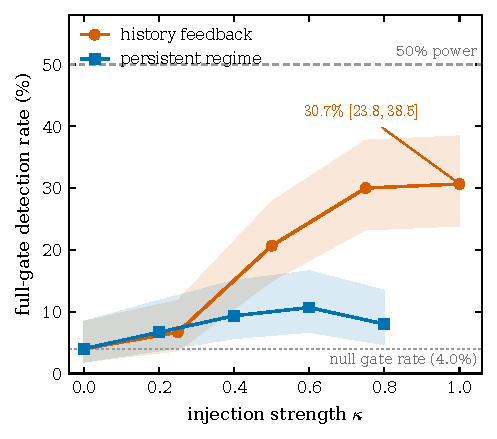
\includegraphics[width=0.65\textwidth]{figS1_mechanism_specific_power.pdf}
\caption{Mechanism-specific sensitivity of the native eight-unit gate. The prespecified alternatives have markedly different detectability; neither grid reaches 50\% power.}
\end{figure}

\section{Near-zero soft-threshold diagnostic}
The $B=249$ operator-ablation analysis in the main paper used $\tau\in\{2,1,0.5,0.25,0.1\}$ and the hard limit. A smaller independently seeded diagnostic extended the path closer to zero with $n=180$ pooled Gaussian trajectories and $B=99$. Table~\ref{tab:nearzero} shows that the transition is gradual rather than discontinuous at $\tau=0$: index rejection and null contraction increase as the soft observable approaches the hard-count geometry, while oracle and native rates remain comparatively stable.

\begin{table}[ht]
\centering
\caption{Near-zero diagnostic for the concentrated profile ($\lambda=4$). The null-SD ratios are medians across trajectories.}\label{tab:nearzero}
\begin{tabular}{rrrrrr}
\toprule
$\tau$ & Oracle rej. & Native rej. & Index rej. & Index-only & SD$_I$/SD$_O$\\
\midrule
0.100 & 3.9\% & 2.2\% & 4.4\% & 2.8\% & 0.846\\
0.050 & 3.3\% & 2.2\% & 3.3\% & 1.7\% & 0.764\\
0.025 & 3.9\% & 2.8\% & 7.8\% & 5.0\% & 0.691\\
0.010 & 4.4\% & 3.9\% & 12.2\% & 8.3\% & 0.583\\
0.005 & 4.4\% & 3.9\% & 12.8\% & 8.9\% & 0.556\\
0.002 & 4.4\% & 3.9\% & 15.0\% & 11.1\% & 0.538\\
0.001 & 4.4\% & 4.4\% & 15.6\% & 11.1\% & 0.538\\
hard & 3.9\% & 3.9\% & 16.1\% & 12.8\% & 0.532\\
\bottomrule
\end{tabular}
\end{table}

\begin{figure}[ht]
\centering
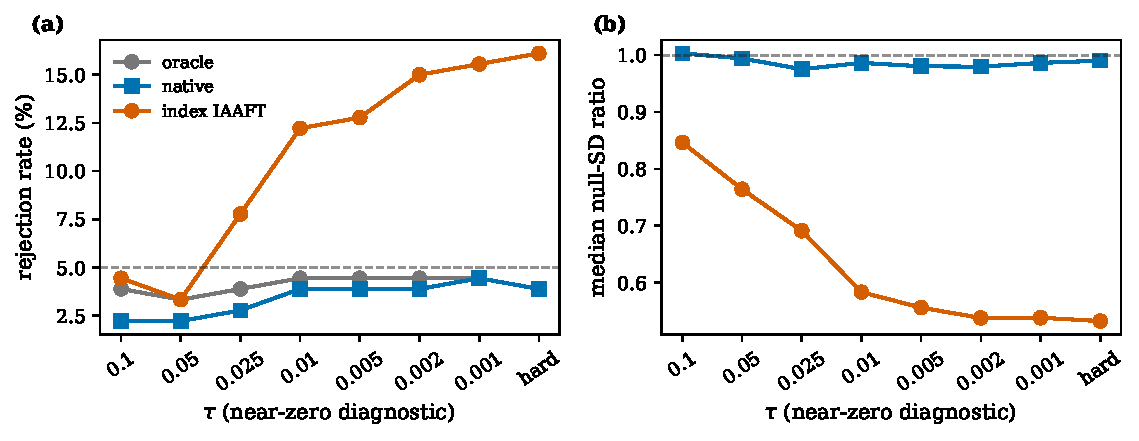
\includegraphics[width=0.78\textwidth]{figS_nearzero_path.pdf}
\caption{Near-zero mechanism diagnostic. (a) Rejection rates as the soft-threshold scale approaches the hard limit. (b) Median native/oracle and index/oracle null-SD ratios. The diagnostic used $B=99$ and is not part of the prespecified benchmark.}
\end{figure}

\section{Extremal-spacing geometry}
In two independently seeded small diagnostics (48 observed trajectories in total; $B=99$ null replicates per trajectory), the hard-count annual IAAFT null regularized the upper-tail spacing relative to oracle and native nulls. At the hard limit, the median ensemble mean number of adjacent exceedance pairs was 2.34 for index IAAFT, 2.89 for native, and 2.88 for oracle. The median inter-exceedance-gap standard deviation was 8.59 for IAAFT and 9.95 for oracle. The corresponding mean Ferro--Segers null was 0.972 for IAAFT, 0.902 for native, and 0.892 for oracle; the null standard deviations were approximately 0.069, 0.132, and 0.132. At $\tau=0.1$, these differences were small. This is the projection through which the lower-tail test becomes more rejection-prone under the annual IAAFT contract.

\section{IAAFT iteration and phase diagnostics}
For the concentrated hard-count condition, the median normalized spectral error was 0.003189 after 10 iterations and 0.002859 after 30, 100, and 300 iterations. For the $\tau=0.01$ soft condition, it was 0.001484 after 30 iterations and 0.001476 after 100 and 300 iterations. Thus the main effect does not arise because 30 iterations stop far from a continuing convergence trajectory.

A global phase-dispersion diagnostic also did not support a simple phase-locking explanation. The median circular resultant of Fourier phases remained close to 0.067--0.069 from the continuous annual mean through near-hard and hard-count conditions. The contraction is therefore more specific to the induced rank/extremal geometry than to global phase collapse.

\section{Within-fiber lumpability diagnostic: detailed summaries}
For each Gaussian AR(1) trajectory $x$, a fiber mate $\widetilde x$ was constructed by permuting exact amplitudes within calendar-month $\times$ threshold-indicator class. Hence $x$ and $\widetilde x$ have identical monthly threshold-indicator sequences, identical annual count sequences, and identical calendar-month empirical value multisets, while generally having different standardized monthly Fourier-amplitude targets. Two independent native ensembles from $x$ provide a same-$x$ Monte Carlo baseline; a third ensemble from $\widetilde x$ provides the within-fiber comparison. Each ensemble used $B=249$, with 90 fiber pairs for each of $\lambda=0$ and $\lambda=4$.

\begin{table}[ht]
\centering
\caption{Within-fiber distributional distances. Distances are Wasserstein distances scaled by the pooled standard deviation of the compared ensembles.}\label{tab:fiber}
\begin{tabular}{lrrrr}
\toprule
Projection & $\lambda$ & Same-$x$ median & Fiber median & Median ratio\\
\midrule
Ferro--Segers & 0 & 0.086 & 0.175 & 1.93\\
Ferro--Segers & 4 & 0.090 & 0.335 & 3.31\\
Lag-1 correlation & 0 & 0.105 & 0.683 & 5.27\\
Lag-1 correlation & 4 & 0.108 & 0.535 & 4.55\\
Raw $T_{\rm diff}$ & 0 & 0.105 & 1.812 & 15.62\\
Raw $T_{\rm diff}$ & 4 & 0.114 & 1.867 & 15.28\\
Low-frequency share & 0 & 0.111 & 0.627 & 5.36\\
Low-frequency share & 4 & 0.099 & 0.379 & 3.97\\
\bottomrule
\end{tabular}
\end{table}

For Ferro--Segers, the fiber distance exceeded the same-$x$ baseline in 73.3\% of pairs at $\lambda=0$ (one-sided sign-test $p=5.45\times10^{-6}$) and 91.1\% at $\lambda=4$ ($p=6.92\times10^{-17}$). KS comparisons rejected equality in 70.0\% of $\lambda=4$ fiber pairs but 1.1\% of same-$x$ controls. For raw $T_{\rm diff}$, all within-fiber pairs were distinguishable by the KS comparison for both seasonal profiles. The hidden target-spectrum separation was larger at $\lambda=4$ than at $\lambda=0$ and was strongly associated with the transported-null distance of $T_{\rm diff}$ (Spearman $\rho\approx0.90$ at $\lambda=4$).


\section{Prospectively frozen SINCA application}
\subsection{Frozen cohort and quality-control screen}
The applied cohort was selected using only station identity, coverage, event-count, and gross scale-quality criteria, before any surrogate $p$-value or null-distribution summary was computed. The fixed analysis window was 2018-01-01 through 2025-12-28 (417 complete weeks). The 31 retained stations span eight regions. Table~\ref{tab:sincacohort} records the exact frozen cohort.

\small
\begin{longtable}{lllrrr}
\caption{Frozen SINCA PM$_{2.5}$ cohort. Coverage is daily coverage over the fixed 2018--2025 window; events are observed days with PM$_{2.5}>50\,\mu$g m$^{-3}$.}\label{tab:sincacohort}\\
\toprule
Station ID & Station & Region & Coverage (\%) & Events & $N_{\mathrm{eff},p}$\\
\midrule
\endfirsthead
\toprule
Station ID & Station & Region & Coverage (\%) & Events & $N_{\mathrm{eff},p}$\\
\midrule
\endhead
RIX/901 & Las Encinas Temuco & IX & 98.7 & 429 & 4.57 \\
RIX/902 & Padre Las Casas II & IX & 99.7 & 668 & 5.41 \\
RIX/905 & Nielol Temuco & IX & 99.9 & 231 & 3.99 \\
RM/D12 & La Florida & RM & 97.9 & 196 & 3.88 \\
RM/D14 & Parque O'Higgins & RM & 98.8 & 210 & 3.65 \\
RM/D15 & Pudahuel & RM & 98.2 & 367 & 3.56 \\
RM/D18 & Cerro Navia & RM & 99.1 & 452 & 3.94 \\
RM/D30 & Quilicura & RM & 99.0 & 257 & 3.49 \\
RVI/609 & Rancagua I & VI & 99.5 & 321 & 3.55 \\
RVI/611 & Rengo & VI & 99.4 & 288 & 3.40 \\
RVI/615 & Rancagua II & VI & 99.7 & 389 & 3.48 \\
RVII/709 & Curicó & VII & 100.0 & 377 & 4.12 \\
RVII/711 & Universidad de Talca & VII & 100.0 & 134 & 3.87 \\
RVIII/802 & Consultorio - San Vicente & VIII & 99.7 & 232 & 4.00 \\
RVIII/804 & JUNJI & VIII & 100.0 & 456 & 4.28 \\
RVIII/806 & Inpesca & VIII & 99.8 & 348 & 4.06 \\
RVIII/810 & INIA. Chillán & VIII & 99.9 & 154 & 4.43 \\
RVIII/832 & Balneario Curanilahue & VIII & 99.9 & 261 & 4.47 \\
RVIII/837 & Nueva Libertad & VIII & 99.2 & 219 & 4.30 \\
RVIII/841 & Hualqui & VIII & 99.2 & 206 & 4.55 \\
RVIII/854 & Punteras & VIII & 99.7 & 105 & 4.85 \\
RVIII/873 & Puren & VIII & 100.0 & 479 & 4.85 \\
RVIII/874 & Los Ángeles Oriente & VIII & 98.3 & 105 & 5.20 \\
RVIII/875 & 21 de mayo & VIII & 99.9 & 432 & 5.21 \\
RX/A01 & Osorno & X & 99.8 & 629 & 5.67 \\
RX/A07 & Mirasol & X & 100.0 & 352 & 5.24 \\
RX/A08 & Alerce & X & 99.6 & 317 & 4.66 \\
RXI/B03 & Coyhaique I & XI & 99.9 & 704 & 5.30 \\
RXI/B04 & Coyhaique II & XI & 100.0 & 749 & 5.32 \\
RXI/B05 & Vialidad & XI & 97.4 & 278 & 4.22 \\
RXIV/E04 & La Union & XIV & 99.1 & 393 & 4.83 \\
\bottomrule
\end{longtable}
\normalsize

\subsection{Applied inferential sensitivity results}
The primary fixed-threshold and probability-equalized results are reported in the main paper. Table~\ref{tab:sincasens} records the prespecified statistic and missingness sensitivities. The exposure-standardized weekly count $7E_w/n_w$ was technically defined for 22 stations; all 22 rejected under the weekly index-level IAAFT null, one rejected under the native transported null, yielding 21 index-only and one joint rejection.

\begin{table}[ht]
\centering
\caption{SINCA sensitivity analyses. Counts are station-level strict $p<0.05$ rejections.}\label{tab:sincasens}
\begin{tabular}{llrr}
\toprule
Threshold branch & Statistic / weekly rule & Index rej. & Native rej.\\
\midrule
Fixed 50 & Ferro--Segers $q=0.90$ & 31/31 & 2/31\\
Fixed 50 & Ferro--Segers $q=0.85$ & 31/31 & 10/31\\
Fixed 50 & normalized $T_{\rm diff}$ & 4/31 & 1/31\\
Fixed 50 & exposure-standardized, FS $q=0.90$ & 22/22 & 1/22\\
Equalized & Ferro--Segers $q=0.90$ & 6/31 & 1/31\\
Equalized & Ferro--Segers $q=0.85$ & 2/31 & 0/31\\
Equalized & normalized $T_{\rm diff}$ & 5/31 & 2/31\\
\bottomrule
\end{tabular}
\end{table}

\subsection{Prespecified null-width mechanism check}
The applied protocol prespecified a positive association between frozen $N_{\mathrm{eff},p}$ and the log null-width ratio
\[
\log R_s=\log\left\{\frac{\mathrm{SD}_{\rm index}}{\mathrm{SD}_{\rm native}}\right\},
\]
corresponding to stronger index-null contraction under more concentrated seasonal event probabilities. The observed Spearman correlation was $-0.379$, with region-cluster bootstrap 95\% interval $[-0.624,0.136]$ (Fig.~\ref{fig:sincawidth}). This prediction was therefore not supported and is reported as such. The primary applied discrepancy instead appears as a large upward displacement of the index-null center.

\begin{figure}[ht]
\centering
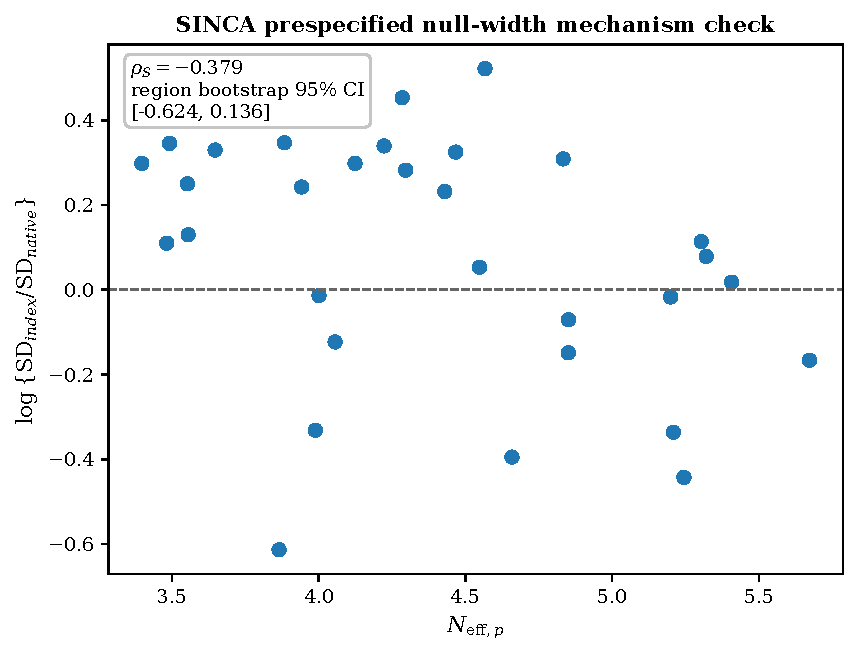
\includegraphics[width=0.65\textwidth]{figS2_sinca_width_mechanism.pdf}
\caption{Prespecified SINCA null-width mechanism check under the fixed $50\,\mu$g m$^{-3}$ threshold. The predicted positive association is not supported. The dashed horizontal line marks equal null standard deviations.}\label{fig:sincawidth}
\end{figure}

\end{document}
